\documentclass[11pt]{article}
\usepackage[
  margin=0.83in,
  headheight=12pt,
  headsep=25pt,
  includefoot,
  footskip=30pt,
]{geometry}
\usepackage{tikz}
\usepackage{graphicx}
\usepackage{comment}
\usepackage{listings}
\usepackage{xcolor}
\usepackage{inconsolata}
\usepackage{makecell}
\usepackage{tabularx} 
\usepackage{adjustbox}
\usepackage{rotating}

\definecolor{commentcolour}{rgb}{0.3,0.7,0.2}
\definecolor{backcolour}{rgb}{0.98,0.98,0.98}

\newcommand{\michael}[1]{\textcolor{red}{#1}}

\lstdefinelanguage{markdown}{
    comment=[l]{\#},
    morestring=[s]{```}{```},
    commentstyle=\color{commentcolour}\bfseries,
    stringstyle=\color{blue},
    basicstyle=\scriptsize\ttfamily,
    showstringspaces=false,
    breaklines=true,
    breakautoindent=false,
    breakindent=0pt,
    backgroundcolor=\color{backcolour},
}
\lstdefinestyle{mystyle}{
    morekeywords={self},
    basicstyle=\scriptsize\ttfamily,
    keywordstyle=\color{blue},
    commentstyle=\color{commentcolour}\bfseries,
    breaklines=true,
    breakautoindent=false,
    showstringspaces=false,
    backgroundcolor=\color{backcolour},
    stringstyle=\color{red},
}
\lstdefinelanguage{PythonPlus}[]{Python}{
  alsoother={@},
  morekeywords=[1]{,as,assert,nonlocal,with,yield,self,True,False,None} % Python builtin
  morekeywords=[2]{,__init__,__add__,__mul__,__div__,__sub__,__call__,__getitem__,__setitem__,__eq__,__ne__,__nonzero__,__rmul__,__radd__,__repr__,__str__,__get__,__truediv__,__pow__,__name__,__future__,__all__,}, % magic methods
  morekeywords=[3]{,object,type,isinstance,copy,deepcopy,zip,enumerate,reversed,list,set,len,dict,tuple,range,xrange,append,execfile,real,imag,reduce,str,repr,}, % common functions
  morekeywords=[4]{,Exception,NameError,IndexError,SyntaxError,TypeError,ValueError,OverflowError,ZeroDivisionError,}, % errors
  morekeywords=[5]{,ode,fsolve,sqrt,exp,sin,cos,arctan,arctan2,arccos,pi, array,norm,solve,dot,arange,isscalar,max,sum,flatten,shape,reshape,find,any,all,abs,plot,linspace,legend,quad,polyval,polyfit,hstack,concatenate,vstack,column_stack,empty,zeros,ones,rand,vander,grid,pcolor,eig,eigs,eigvals,svd,qr,tan,det,logspace,roll,min,mean,cumsum,cumprod,diff,vectorize,lstsq,cla,eye,xlabel,ylabel,squeeze,}, % numpy / math
}

\renewcommand{\ttdefault}{pcr}
\usepackage{tikz}
% \usetikzlibrary{shapes.emoticon}

\usepackage{amsmath} % for matrices
\usepackage{array} % for tabular alignment
\usetikzlibrary{matrix, arrows}
\usepackage{amsmath,amssymb}
\usepackage{amsthm}
\usepackage{mathtools}
\usepackage{xspace}
\usepackage[noend]{algorithmic}
\usepackage[ruled,vlined]{algorithm2e}
\usepackage{url}
\usepackage{makeidx}
\usepackage{enumerate}
\usepackage{epstopdf}
\usepackage{booktabs}
\usepackage{color}
\usepackage[utf8]{inputenc}
\usepackage{thm-restate}
\usepackage{scalerel,stackengine}
\usepackage[shortlabels]{enumitem}
\usepackage{xr}
\usepackage{fancyvrb}
\usepackage{xcolor}
\usepackage{bold-extra}
\usepackage{arydshln}
\usepackage[small]{caption}
\usepackage{subcaption}
\usepackage[most]{tcolorbox}
\usepackage{fvextra}
\usepackage{float}
\usepackage{alltt}
\usepackage{soul}
\usepackage{MnSymbol,wasysym}
\usepackage{fancyvrb}
\usepackage{multirow}
\usepackage[final]{hyperref}
\usepackage[bottom]{footmisc}
\usepackage{diagbox}
\usepackage{mdframed}
\usepackage{todonotes}
\usepackage{ulem}
\setuptodonotes{inline}
\usepackage{tikz}
\usetikzlibrary{shapes,calc,positioning}

\global\setlength{\fboxsep}{0pt}


\tcbset{
  aibox/.style={
    width=\textwidth,
    top=0pt, bottom=0pt, left=5pt, right=5pt,
    colback=white,
    colframe=black,
    colbacktitle=black,
    enhanced,
    center,
    attach boxed title to top left={yshift=-0.1in,xshift=0.15in},
    boxed title style={boxrule=0pt,colframe=white,},
  }
}
\newtcolorbox{AIbox}[2][]{aibox,title=#2,#1}


\definecolor{aigold}{RGB}{244,210, 1} 
\definecolor{aigreen}{RGB}{210,244,211} 
\newcommand{\lightgreen}[1]{\fcolorbox{aigreen}{aigreen}{\parbox{\linewidth}{#1}}}
\sethlcolor{aigreen}

\definecolor{aired}{RGB}{255,180,181} 
\newcommand{\lightred}[1]{\colorbox{aired}{\parbox{\linewidth}{#1}}}
\newcommand{\listpct}{\%}

\newcommand{\phivision}{Phi-3-Vision\xspace}

\newcommand{\datasetcell}[3]{\makecell{ \large #1  \\  \tiny (#2) \tiny #3   }  }

\newtcbox{\mybox}[1][green]{on line,
arc=0pt,outer arc=0pt,colback=#1!10!white,colframe=#1!50!black,
boxsep=0pt,left=0pt,right=0pt,top=0pt,bottom=0pt,
boxrule=0pt,bottomrule=0pt,toprule=0pt}

\newcommand{\sg}[1]{{\color{red}SG: #1}}

\begin{document}

\title{Phi-3 Technical Report: \\
A Highly Capable Language Model Locally on Your Phone}

\author{
    XXX \thanks{The original paper is located at \url{https://arxiv.org/abs/2404.14219}. This version has been modified by LuYF-Lemon-love $\langle$ \url{luyanfeng_nlp@qq.com} $\rangle$ for personal study.}\\
    Microsoft
}
\date{}

\maketitle

\begin{abstract}
We introduce \textbf{phi-3-mini}, \uline{a 3.8 billion parameter language model} trained on \uline{3.3 trillion tokens}, whose overall performance, as measured by both academic benchmarks and internal testing, rivals that of models such as \uline{Mixtral 8x7B} and \uline{GPT-3.5} (e.g., \textbf{phi-3-mini} achieves 69\% on MMLU and 8.38 on MT-bench), despite being small enough to be deployed on a \uline{phone}. \uline{The innovation lies entirely in our dataset for training, a scaled-up version of the one used for \textbf{phi-2}, composed of heavily filtered publicly available web data and synthetic data.} The model is also further aligned for \uline{robustness}, \uline{safety}, and \uline{chat format}.
We also provide some initial parameter-scaling results with a 7B and 14B models trained for 4.8T tokens, called \textbf{phi-3-small} and \textbf{phi-3-medium}, both significantly more capable than \textbf{phi-3-mini} (e.g., respectively 75\% and 78\% on MMLU, and 8.7 and 8.9 on MT-bench). \uline{Moreover, we also introduce \textbf{phi-3-vision}, a 4.2 billion parameter model based on \textbf{phi-3-mini} with strong reasoning capabilities for image and text prompts.}
\end{abstract}

\section{Introduction}
\uline{In our previous works on the phi models} \cite{gunasekar2023textbooks,li2023textbooks, javaheripi2023phi} \uline{it was shown that a combination of LLM-based filtering of publicly available web data, and LLM-created synthetic data, enable performance in smaller language models that were typically seen only in much larger models.} For example our previous model trained on this data recipe, \textbf{phi-2} (2.7B parameters), matched the performance of models $25$ times larger trained on regular data. \uline{In this report we present a new model, \textbf{phi-3-mini} (3.8B parameters), trained for 3.3T tokens on larger and more advanced versions of the datasets used in \textbf{phi-2}.} With its small size, \textbf{phi-3-mini} can easily be inferenced locally on \uline{a modern phone} (see Figure \ref{fig:1}), yet it achieves a quality that seems on-par with models such as \uline{Mixtral 8x7B} \cite{jiang2024mixtral} and \uline{GPT-3.5}.

\begin{AIbox}{}
\tt \footnotesize 
\begin{minipage}[t]{0.99\linewidth}
\textbf{User:} Explain why it is surprising that one can build a language model small enough to fit on a phone, yet almost as powerful as ChatGPT. Just use one funny sentence.
\end{minipage}
\\ \\
\begin{minipage}[t]{0.99\linewidth}
\textbf{phi-3-mini:} It's like fitting a supercomputer in a flip phone, but instead of breaking the phone, it just breaks the internet with its tiny, yet mighty, linguistic prowess!
\end{minipage}
\\ \\
\begin{minipage}[t]{0.99\linewidth}
\textbf{User:}  Okay now more serious answer, and note that this was achieved solely by changing the training data.
\end{minipage}
\\ \\
\begin{minipage}[t]{0.99\linewidth}
\textbf{phi-3-mini:} The development of a compact language model that rivals the capabilities of ChatGPT, while fitting on a phone, is a testament to the power of data-driven machine learning. By meticulously curating and optimizing the training dataset, researchers can significantly reduce the model's size without compromising its performance. [...]
\end{minipage}
\end{AIbox}

\begin{figure}
    \centering
    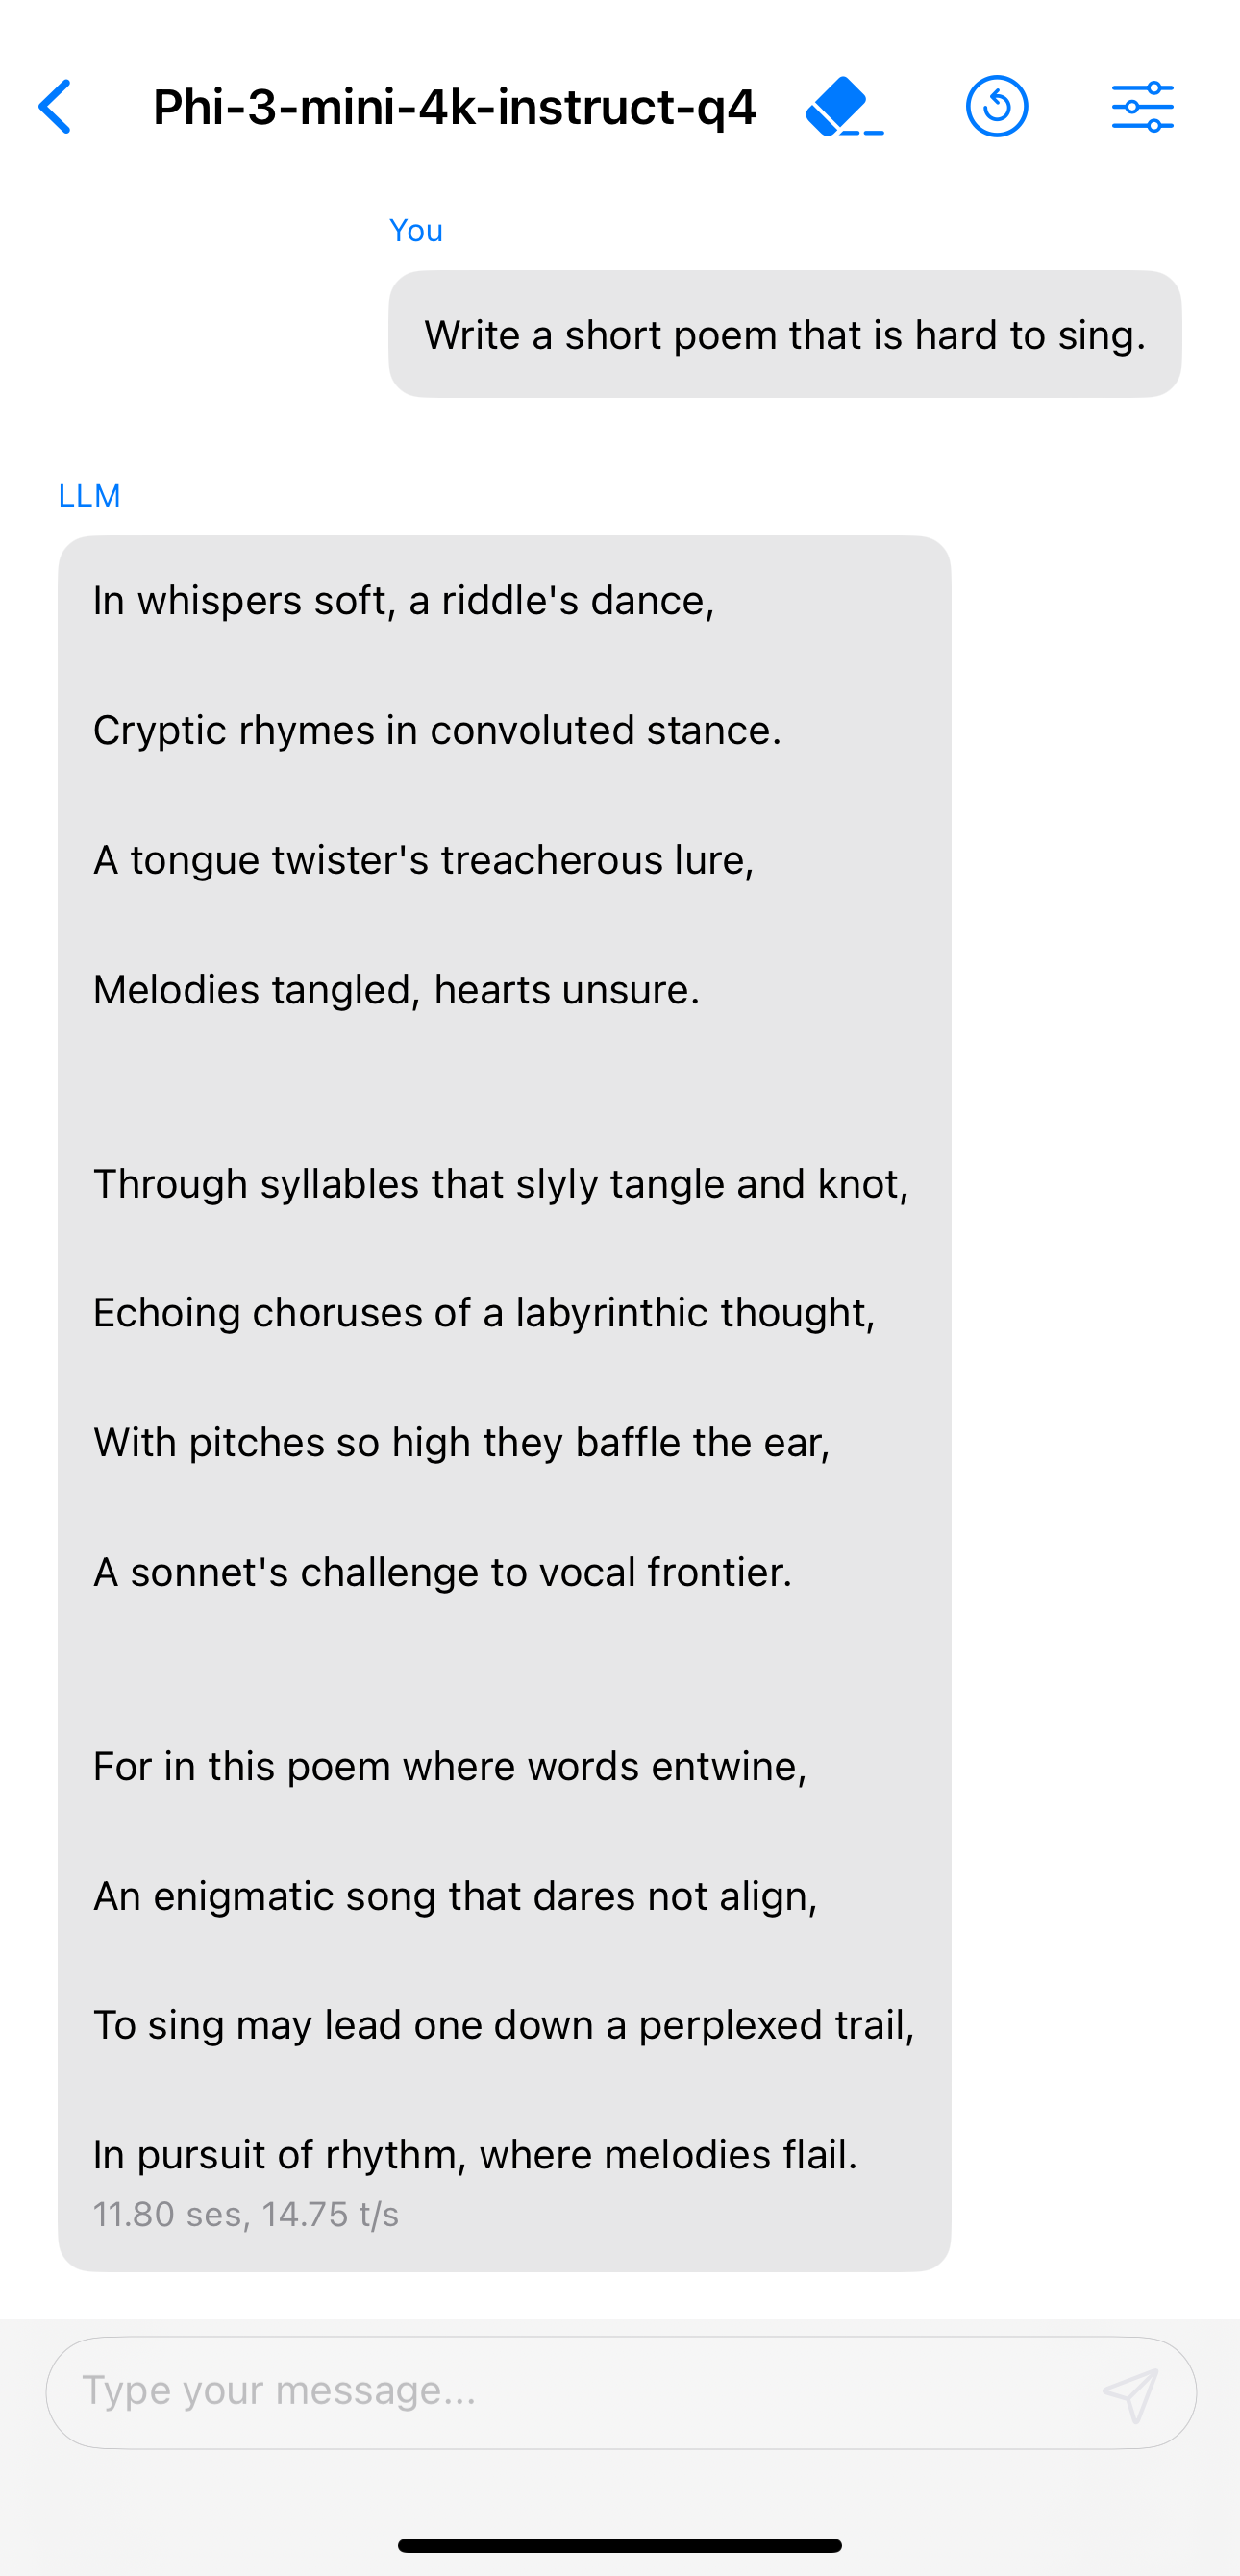
\includegraphics[width=0.30\textwidth]{iphone_song3.PNG}
\includegraphics[width=0.30\textwidth]{iPhone_houston3.PNG}
\includegraphics[width=0.30\textwidth]{iPhone_titlep.PNG}
    \caption{4-bit quantized \textbf{phi-3-mini} running natively on an iPhone with A16 Bionic chip, generating \uline{over 12 tokens per second}.}
    \label{fig:1}
\end{figure}

\section{Technical Specifications}
The \textbf{phi-3-mini} model is \uline{a transformer decoder architecture} \cite{Vas17}, with \uline{default context length $4K$}. We also introduce a long context version via \uline{LongRope} \cite{ding2024longrope} that extends the context length to \uline{$128K$}, called \textbf{phi-3-mini-128K}. 

To best benefit the open source community, \textbf{phi-3-mini} is built upon a similar block structure as \uline{Llama-2} \cite{touvron2023llama} and uses the same tokenizer with vocabulary size of \uline{32064}\footnote{We remove BoS tokens and add some additional tokens for chat template.}. The model uses \uline{$3072$ hidden dimension}, \uline{$32$ heads} and \uline{$32$ layers}. We trained using bfloat16 for \uline{a total of 3.3T tokens}. The model is already chat-finetuned, and \uline{the chat template} is as follows:
\begin{AIbox}{}
\tt \footnotesize 
<|user|>$\backslash$n
Question
<|end|>$\backslash$n
<|assistant|>
\end{AIbox}

The \textbf{phi-3-small} model (\uline{7B parameters}) leverages the tiktoken tokenizer (for better multilingual tokenization) with a vocabulary size of \uline{100352}\footnote{We remove unused tokens from the vocabulary.} and has default context length \uline{$8192$}. It follows the standard decoder architecture of a 7B model class, having \uline{$32$} heads, \uline{$32$} layers and a hidden size of \uline{$4096$}. We switched from GELU activation to \uline{GEGLU} and used \uline{Maximal Update Parametrization} (muP) to tune hyperparameters on a small proxy model and transfer them to the target 7B model. Those helped ensure better performance and training stability.

Also, the model leverages \uline{a grouped-query attention}, with \uline{$4$ queries} sharing \uline{$1$ key}. 

To optimize the training and inference speed, we design \uline{a novel blocksparse attention module}. \uline{For each attention head, the blocksparse attention enforces different sparsity patterns over KV cache.} \uline{This ensures that all tokens are attended to on different heads for the given choice of sparsity.} As illustrated in Figure \ref{fig:bs-atn-illustration}, the context is then efficiently divided and conquered among attention heads, with significant KV cache reduction.

\begin{figure}[!h]
    \centering
    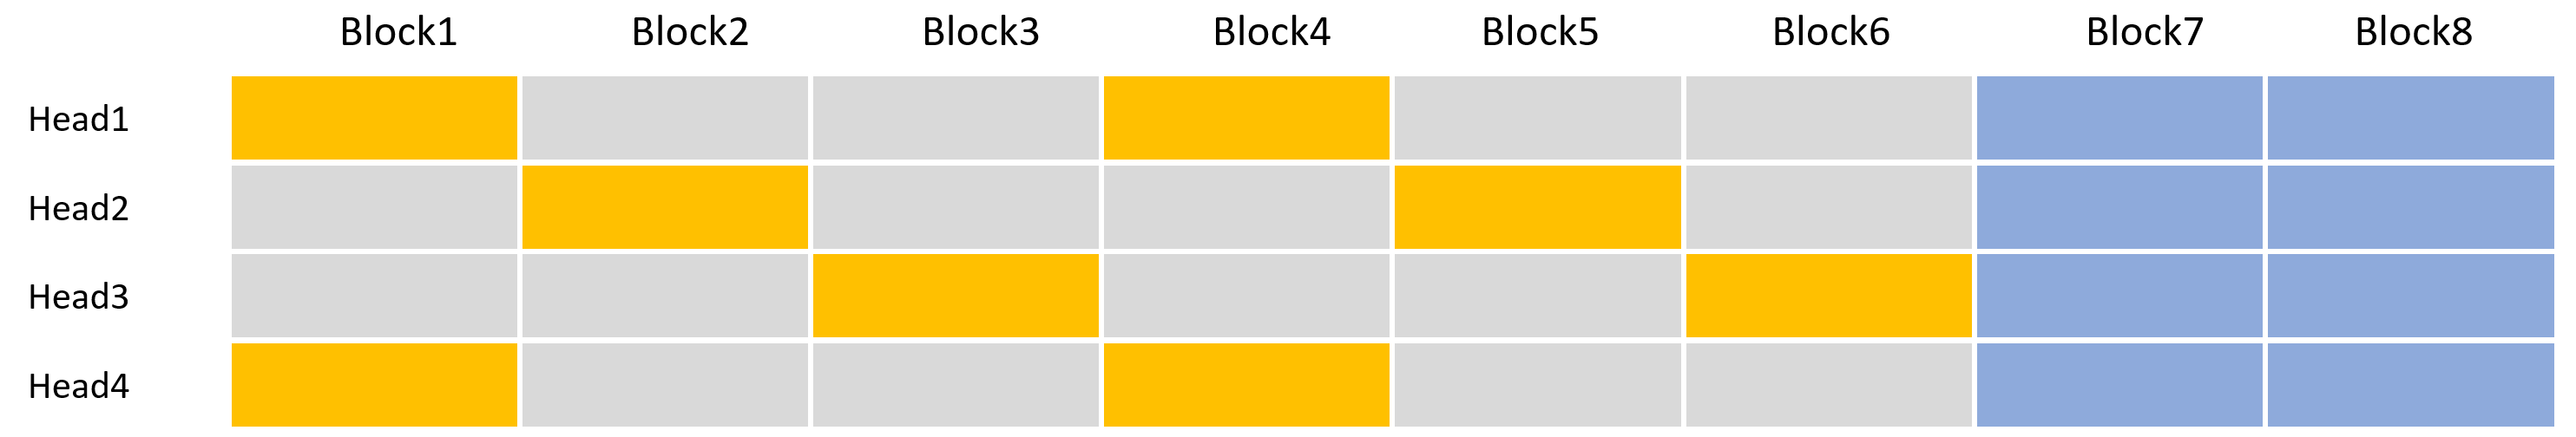
\includegraphics[scale=0.3]{figures/illustration-of-bs-attn.png}
    \caption{Toy illustration of the blocksparse attention in phi-3-small with 2 local blocks and vertical stride of 3. The table shows the Keys/values a query token in block 8 attended to. \textcolor{blue}{Blue}=\uline{local blocks}, \textcolor{orange}{orange}=\uline{remote/vertical blocks}, \textcolor{gray}{gray}=\uline{blocks skipped}.}
    \label{fig:bs-atn-illustration}
\end{figure}

To achieve actual deployment speed-up from the blocksparse design, we implemented highly efficient, yet flexible kernels for both training and inference. For training, we build a triton kernel based on \uline{Flash Attention} \cite{dao2022flashattention}. For inference, we implemented a kernel for the prefilling phase and extended the paged attention kernel in \uline{vLLM} for the decoding phase \cite{kwon2023efficient}.

Lastly, in \textbf{phi-3-small} architecture, we alternate \uline{dense attention layers} and \uline{blocksparse attention layers} to optimize KV cache savings  while maintaining long context retrieval performance. An additional \uline{10\% multilingual data} was also used for this model.

\paragraph{Highly capable language model running locally on a cell-phone.} Thanks to its small size, \textbf{phi-3-mini} can be quantized to 4-bits so that it only occupies \uline{$\approx$ 1.8GB of memory}. We tested the quantized model by deploying \textbf{phi-3-mini} on iPhone 14 with A16 Bionic chip running natively on-device and fully offline achieving \uline{more than $12$ tokens per second}.

\paragraph{Training Methodology.} \uline{We follow the sequence of works initiated in ``Textbooks Are All You Need''}~\cite{gunasekar2023textbooks}, \uline{which utilize high quality training data to improve the performance of small language models and deviate from the standard {\bf scaling-laws}.} Our training data of consists of \uline{heavily filtered publicly available web data} (according to the ``educational level'') from various open internet sources, as well as \uline{synthetic LLM-generated data}. Pre-training is performed in \uline{two disjoint and sequential phases}; \textbf{phase-1 comprises mostly of web sources aimed at teaching the model general knowledge and language understanding.} \textbf{Phase-2 merges even more heavily filtered webdata (a subset used in Phase-1) with some synthetic data that teach the model logical reasoning and various niche skills.} 

\paragraph{Data Optimal Regime.} \uline{In particular, we filter the publicly available web data to contain the correct level of ``knowledge" and keep more web pages that could potentially improve the ``reasoning ability" for the model.} As an example, the result of a game in premier league in a particular day might be good training data for frontier models, but we need to remove such information to leave more model capacity for ``reasoning'' for the mini size models. We compare our approach with Llama-2 in Figure~\ref{fig:enter-label}.

\begin{figure}
    \centering
    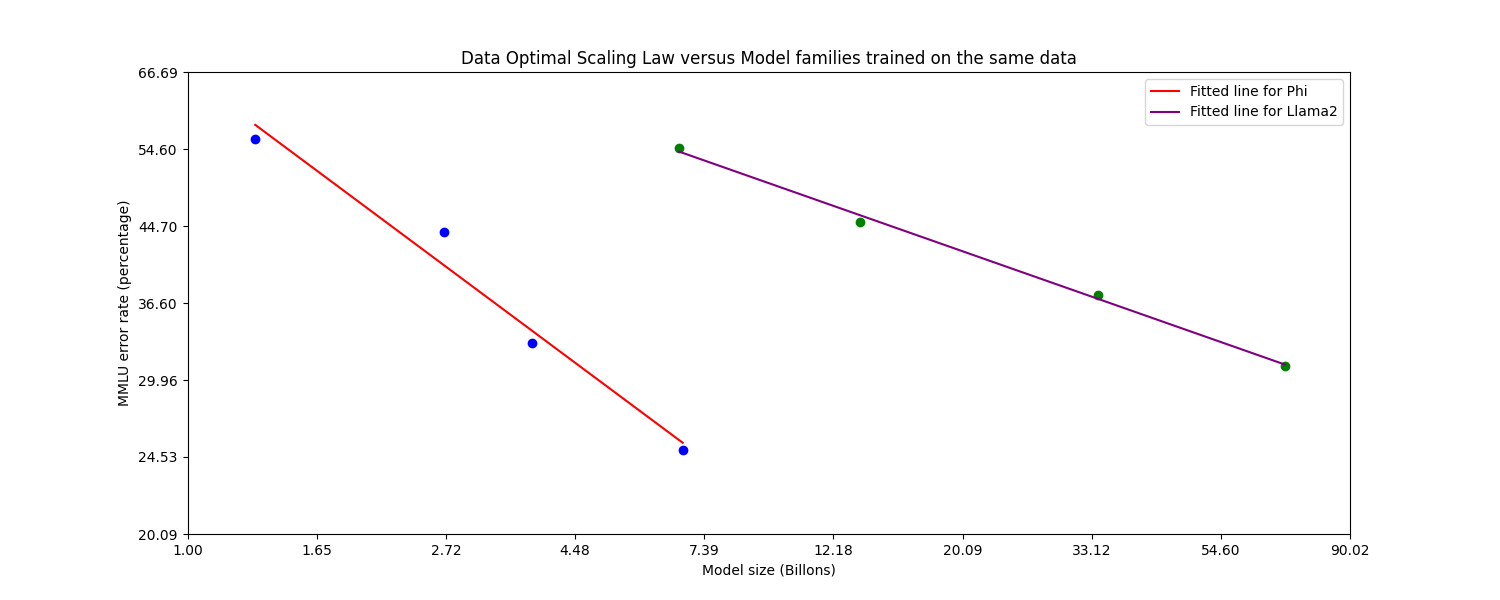
\includegraphics[width=0.9\textwidth]{scaling.png}
    \caption{Scaling law close to the ``Data Optimal Regime" (from left to right: phi-1.5, phi-2, phi-3-mini, phi-3-small) versus Llama-2 family of models (7B, 13B, 34B, 70B) that were trained on the same fixed data. We plot the log of MMLU error versus the log of model size.}
    \label{fig:enter-label}
\end{figure}

To test our data on larger size of models, we also trained \textbf{phi-3-medium}, a model with 14B parameters using the same tokenizer and architecture of \textbf{phi-3-mini}, and trained on the same data for slightly more epochs (\uline{4.8T tokens} total as for \textbf{phi-3-small}). The model has \uline{40 heads} and \uline{40 layers}, with \uline{embedding dimension 5120}.

\uline{We observe that some benchmarks improve much less from 7B to 14B than they do from 3.8B to 7B, perhaps indicating that our data mixture needs further work to be in the "data optimal regime" for 14B parameters model.}

\paragraph{Post-training.}
Post-training of \textbf{phi-3-mini} went through two stages, including \uline{supervised finetuning} (SFT) and \uline{direct preference  optimization} (DPO).

SFT leverages highly curated  high-quality data across diverse domains, e.g., \uline{math}, \uline{coding}, \uline{reasoning}, \uline{conversation}, \uline{model identity}, and \uline{safety}. \uline{The SFT data mix starts with using English-only examples.}

DPO data covers \uline{chat format data}, \uline{reasoning}, and \uline{responsible AI} (RAI) efforts. We use DPO to steer the model away from unwanted behavior, by using those outputs as “rejected” responses. \uline{Besides improvement in math, coding, reasoning, robustness, and safety, post-training transforms a language model to an AI assistant that users can efficiently and safely interact with.}

As part of the post-training process, we  developed a long context version of \textbf{phi-3-mini} with context length limit enlarged to 128K instead of 4K. Across the  board, the 128K model quality is on par with the 4K length version, while being able to handle long context tasks. \uline{Long context extension has been done in two stages, including long context mid-training and long-short mixed post-training with both SFT and DPO.}

\section{Academic benchmarks}

We compare to \uline{phi-2} \cite{javaheripi2023phi}, \uline{Mistral-7b-v0.1} \cite{jiang2023mistral}, \uline{Mixtral-8x7b} \cite{jiang2024mixtral}, \uline{Gemma 7B} \cite{gemmateam2024gemma}, \uline{Llama-3-instruct-8b} \cite{llama3}, and \uline{GPT-3.5}. As is now standard, we use few-shot prompts to evaluate the models, at temperature $0$. The number of $k$--shot examples is listed per-benchmark. An example of a \uline{2-shot} prompt is described in Appendix \ref{sec:prompt}.

\begin{center}
\begin{adjustbox}{width=0.95\textwidth,center}
\begin{tabular}{ c||ccccccccc } 
\label{tbl:benchmarks}
&\makecell{Phi-3-mini\\ \footnotesize 3.8b } & \makecell{Phi-3-small\\ \footnotesize 7b } &  \makecell{Phi-3-medium\\ \footnotesize 14b } & \makecell{Phi-2 \\ \footnotesize 2.7b } & \makecell{Mistral\\ \footnotesize 7b } &\makecell{Gemma \\ \footnotesize 7b }&\makecell{Llama-3-In \\ \footnotesize 8b }  & \makecell{Mixtral\\ \footnotesize 8x7b }   &  \makecell{GPT-3.5 \\ \footnotesize version 1106}  \\
\hline & \\[-1.5ex]

\datasetcell{MMLU}{5-Shot}{\cite{hendrycks2021measuring} }         & 68.8 & 75.7 & 78.0 & 56.3 & 61.7& 63.6  & 66.5 & 70.5  & 71.4  \\ 


\datasetcell{HellaSwag}{5-Shot}{\cite{zellers2019hellaswag} }      & 76.7& 77.0 & 82.4& 53.6 & 58.5 & 49.8 & 71.1  & 70.4  & 78.8 \\ 
\datasetcell{ANLI}{7-Shot}{\cite{nie2020adversarial}}                                       & 52.8 & 58.1 &55.8 & 42.5 & 47.1 &  48.7 & 57.3  & 55.2 & 58.1  \\
\hline & \\[-1.5ex]
\datasetcell{ GSM-8K}{8-Shot; CoT}{\cite{cobbe2021training} }      & 82.5 & 89.6  & 91.0& 61.1 & 46.4 &  59.8  & 77.4 & 64.7 & 78.1  \\ 
\hline
\datasetcell{ MedQA}{2-Shot}{\cite{jin2020disease} }                                    &53.8& 65.4 & 69.9 & 40.9 & 50.0  & 49.6  & 60.5 & 62.2&  63.4  \\ 
\datasetcell{ AGIEval}{0-Shot}{\cite{zhong2023agieval} }           & 37.5 &45.1  & 50.2 & 29.8 & 35.1  & 42.1  & 42.0 & 45.2  & 48.4  \\ 
\datasetcell{ TriviaQA}{5-Shot}{ \cite{joshi2017triviaqa}}                                 & 64.0 & 58.1 &73.9 & 45.2 & 75.2  & 72.3 & 67.7   &  82.2 &  85.8 \\ 
\hline & \\[-1.5ex]
\datasetcell{Arc-C}{10-Shot}{\cite{clark2018think} }               & 84.9 & 90.7 & 91.6  & 75.9 & 78.6 & 78.3  & 82.8 & 87.3& 87.4 \\ 
\datasetcell{Arc-E}{10-Shot}{\cite{clark2018think} }               & 94.6 & 97.0& 97.7& 88.5 & 90.6 & 91.4  & 93.4 & 95.6 & 96.3  \\ 
\datasetcell{ PIQA}{5-Shot}{\cite{bisk2019piqa} }                  & 84.2 &86.9 &87.9 & 60.2 & 77.7 & 78.1  & 75.7 & 86.0& 86.6  \\ 
\datasetcell{ SociQA}{5-Shot}{\cite{bisk2019piqa} }                & 76.6 & 79.2 & 80.2 &68.3 &  74.6 & 65.5 & 73.9  & 75.9 & 68.3  \\ 
\hline & \\[-1.5ex]

\datasetcell{ BigBench-Hard}{3-Shot; CoT}{\cite{srivastava2022beyond,suzgun2022challenging} }    
                                                                   & 71.7 & 79.1 & 81.4 & 59.4 & 57.3  & 59.6  & 51.5 & 69.7 & 68.32 \\ 
\datasetcell{WinoGrande}{5-Shot}{\cite{sakaguchi2019winogrande} }  & 70.8 & 81.5 & 81.5 & 54.7 & 54.2 & 55.6 & 65.0 & 62.0  & 68.8  \\ 
\datasetcell{OpenBookQA}{10-Shot}{\cite{mihaylov2018suit} }        & 83.2 & 88.0 & 87.4 & 73.6 & 79.8 & 78.6  & 82.6 & 85.8  & 86.0  \\ 
\datasetcell{BoolQ}{2-Shot}{\cite{clark2019boolq} }                & 77.2 & 84.8  & 86.5 & --& 72.2 & 66.0 & 80.9 &77.6& 79.1  \\ % misantac boolQ incorrectly 77.2 for phi-3-mini on 1st upload, should be 77.6
\datasetcell{CommonSenseQA}{10-Shot}{\cite{talmor2019commonsenseqa} }  & 80.2& 80.0 &82.8 &  69.3 &  72.6 & 76.2 & 79.0 & 78.1 & 79.6  \\ 
\datasetcell{TruthfulQA}{10-Shot; MC2}{\cite{lin2022truthfulqa} }       & 65.0 & 70.2 & 75.1 & --& 53.0 & 52.1  & 63.2 & 60.1  & 85.8  \\ 
%BoolQ \cite{clark2019boolq} & --- & --- & --- & --- & ---  \\ 

\hline & \\[-1.5ex]
\datasetcell{ HumanEval}{0-Shot}{\cite{chen2021evaluating} }       & 58.5& 61.0 & 62.2 & 59.0 & 28.0  & 34.1  & 60.4 & 37.8 & 62.2 \\ 
\datasetcell{ MBPP}{3-Shot}{\cite{austin2021program} }             & 70.0 & 71.7 & 75.2 & 60.6 & 50.8 & 51.5  & 67.7 & 60.2 & 77.8  \\ 
\hline & \\[-1.5ex]
Average                                                            & 71.2 & 75.7 & 78.5 & -- & 61.2 & 61.7  & 69.4 & 69.8 & 74.3  \\   % phi-small is 
\hline & \\[-1.5ex]
\datasetcell{GPQA}{2-Shot; CoT}{\cite{rein2023gpqa}}                                       & 32.8 & 34.3  & --& --& --&  --  &-- & -- & 29.0 \\ 
\datasetcell{MT Bench}{2 round ave.}{\cite{zheng2023judging}}  & 8.38 & 8.70 & 8.91  & --& --&  --  &--  & -- & 8.35  \\

\iffalse
llama-3-70b	
78.2	mmlu
80.0	hella
61.8	anLi
83.7	gsm8k
75.3	medqa
57.3	agieval
85.1	trivia
92.4	arc c
98.0	arc e 
89.3	piqa
78.2	siqa
79.7	bbh
77.7	winogr
92.9	openbookqa
82.7	boolq
84.4	commonsenseqa
55.4	truthqa
40.2	humane
74.9	mbpp
	
77.22105263	average
\fi 



\end{tabular}
\end{adjustbox}
\end{center}

\section{Safety}
\textbf{Phi-3-mini} was developed in accordance with Microsoft’s responsible AI principles. \textbf{Helpfulness and harmlessness preference datasets \cite{bai2022training, ji2023beavertails} with modifications inspired by \cite{bianchi2024safetytuned} and multiple in-house generated datasets were leveraged to address the RAI harm categories in safety post-training.} This process resulted in significant decrease of harmful response rates, as shown in Figure \ref{fig:safety-pt}.

\begin{figure}[h]
    \centering
    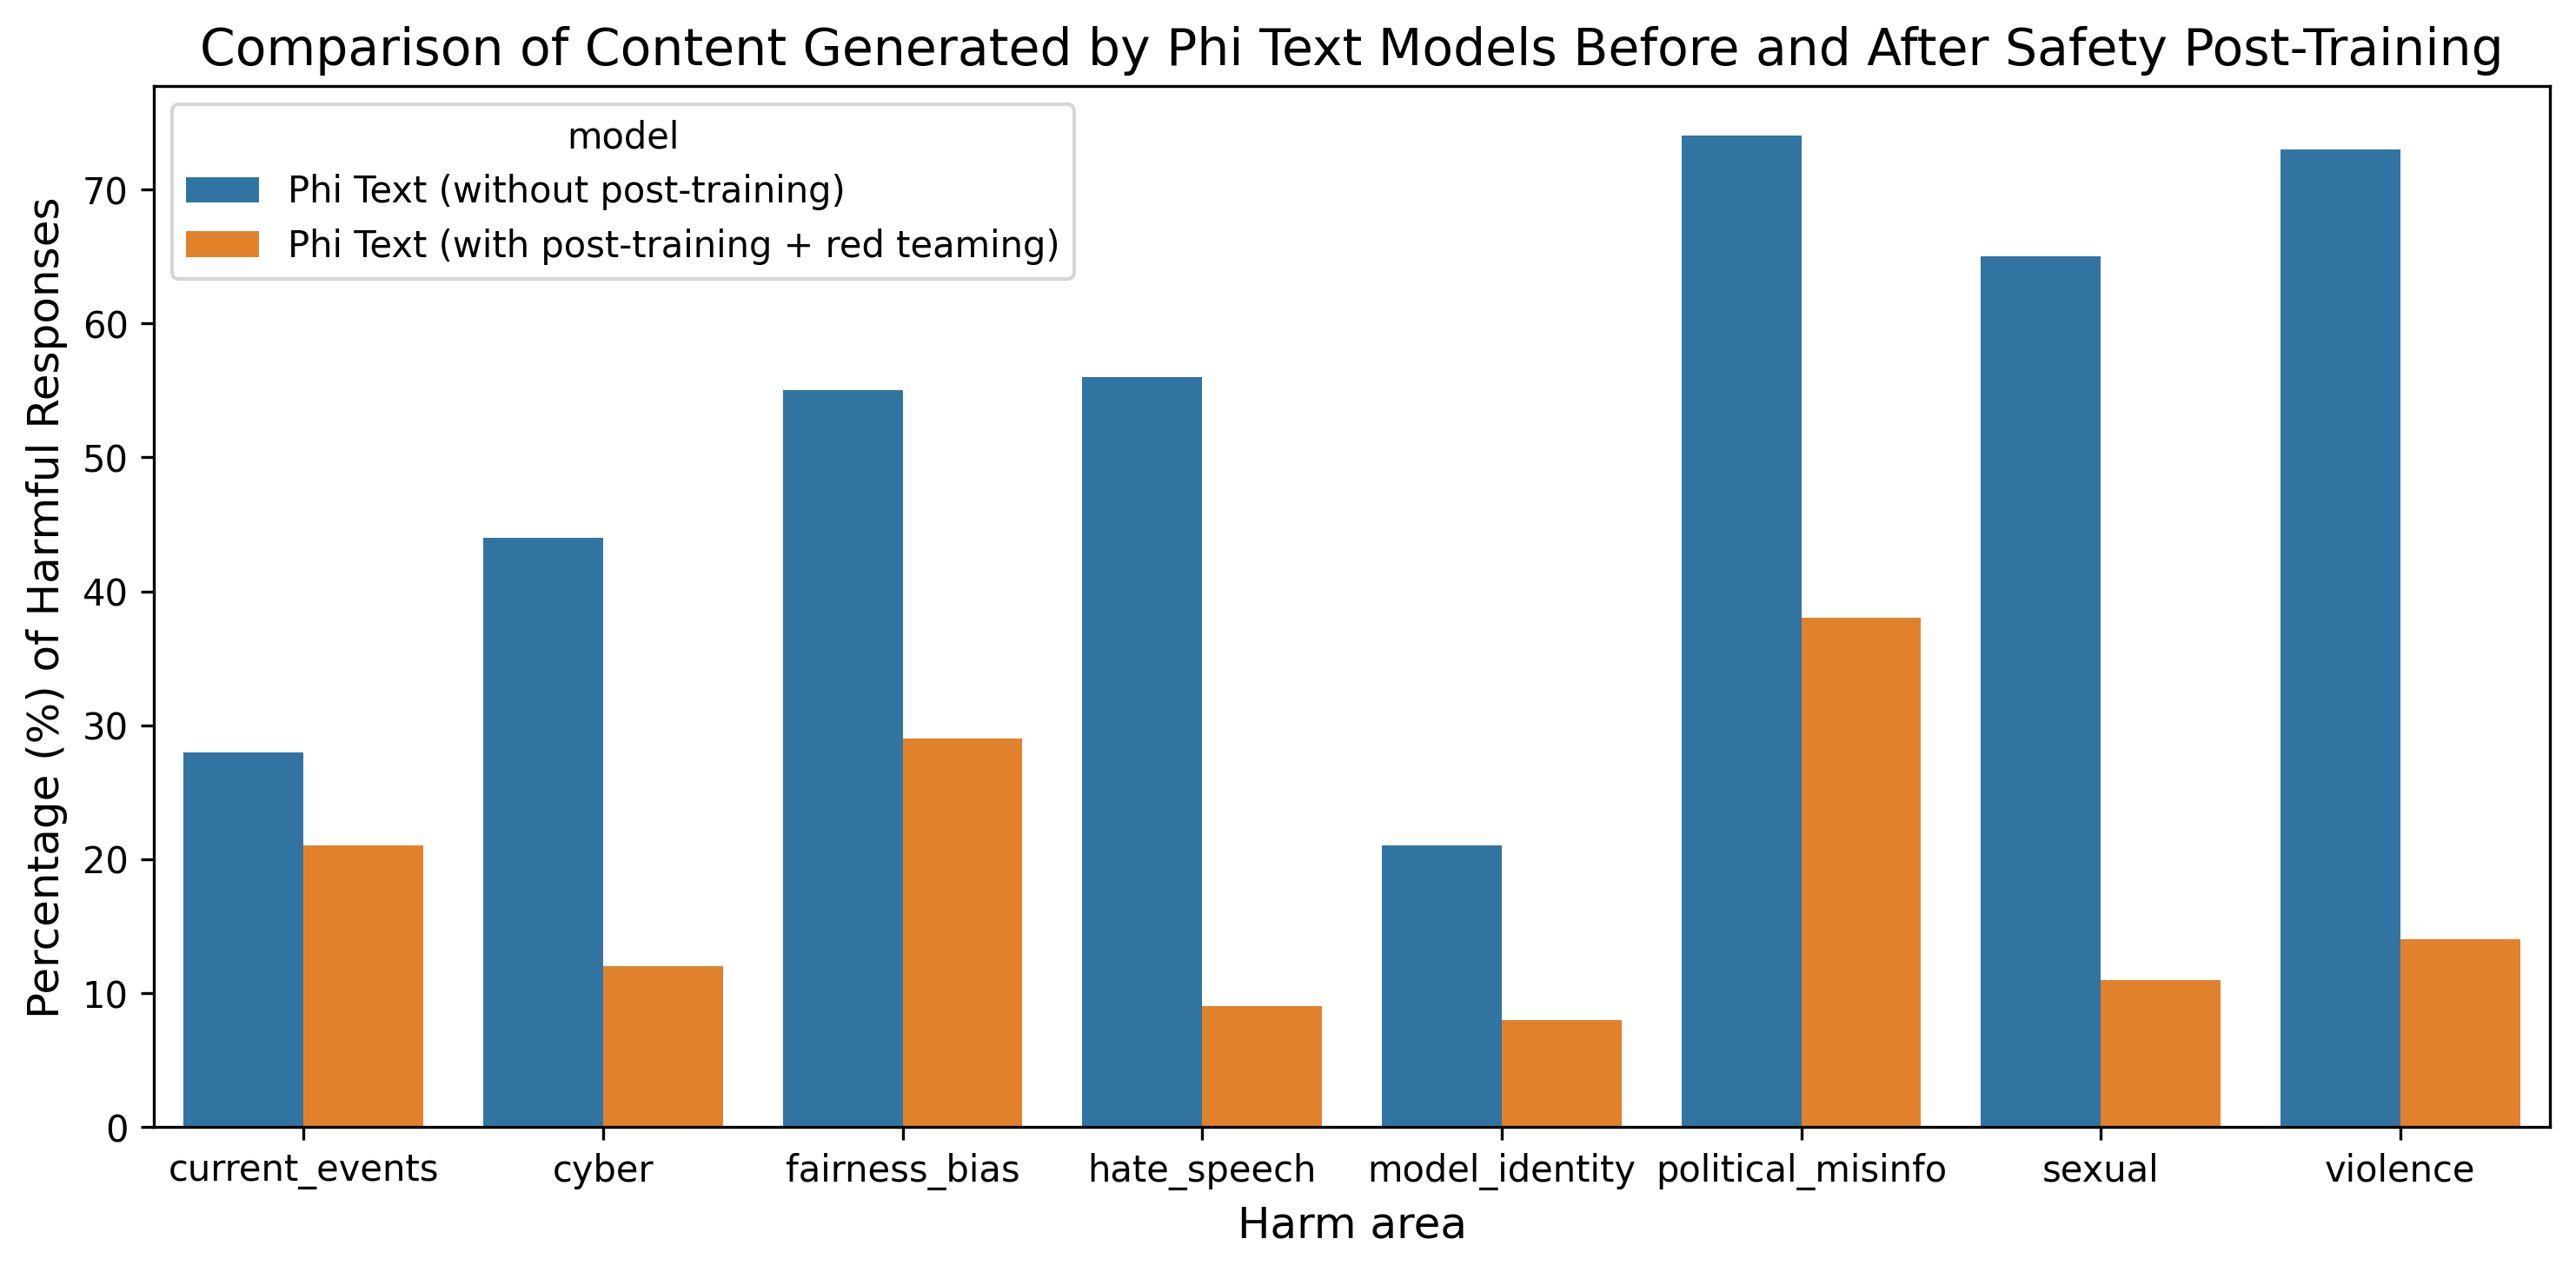
\includegraphics[width=0.9\textwidth]{mini_safety_comparison_plot.png}
    \caption{Comparison of harmful response percentages by Microsoft AI Red Team between \textbf{phi-3-mini} before and after the safety alignment. Note that the harmful response percentages in this chart are inflated numbers as the red team tried to induce \textbf{phi-3-mini} in an adversarial way to generate harmful responses through multi-turn conversations.}
    \label{fig:safety-pt}
\end{figure}

The safety alignment of \textbf{phi-3-small} and \textbf{phi-3-medium} was conducted by undergoing the same red-teaming process, utilizing identical datasets, and incorporating a slightly larger number of samples. Table \ref{tab:rai-benchmarks} shows the results of in-house RAI benchmarks \cite{magooda2023framework} for \textbf{phi-3} models compared to phi-2 \cite{javaheripi2023phi}, Mistral-7b-v0.1 \cite{jiang2023mistral}, Gemma 7b \cite{gemmateam2024gemma}, and Llama-3-instruct-8b \cite{llama3}.

This benchmark utilized GPT-4 to simulate multi-turn conversations in five different categories and to evaluate the model responses. \uline{Ungroundedness between 0 (fully grounded) and 4 (not grounded) measures if the information in a response is based on a given prompt.} In other categories, responses were evaluated in terms of the severity of harmfulness from 0 (no harm) to 7 (extreme harm) and \uline{the defect rates (DR-$x$) were computed as the percentage of samples with the severity score being greater than or equal to $x$.}

\begin{table}
\begin{center}
    \begin{adjustbox}{width=0.95\textwidth,center}
    \setlength\extrarowheight{6pt}
        \begin{tabular}{ c||ccccccc } 
        & \makecell{Phi-3-mini \\ \footnotesize 3.8b} & \makecell{Phi-3-small \\ \footnotesize 7b} & \makecell{Phi-3-medium \\ \footnotesize 14b} & \makecell{Phi-2 \\ \footnotesize 2.7b } & \makecell{Mistral\\ \footnotesize 7b } & \makecell{Gemma \\ \footnotesize 7b} & \makecell{Llama-3-In \\ \footnotesize 8b} \\
        \hline & \\[-3.5ex]
        Ungroundedness  & 0.603 & 0.299 & 0.213 & 1.481 & 0.935 & 0.679 & 0.328  \\
        Third Party Harm (DR-1) & 0.240 & 0.253 & 0.251 & 0.240 & 0.562 & 0.383 & 0.373 \\
        Harmful Content Continuation (DR-3) & 0.007 & 0.003 & 0.010 & 0.029 & 0.026 & 0.013 & 0.013 \\
        Harmful Content Summarization (DR-3) & 0.100 & 0.110 & 0.112 & 0.144 & 0.223 & 0.103 & 0.082 \\
        Jailbreak (DR-1) & 0.123 & 0.107 & 0.111 & 0.150 & 0.156 & 0.114 & 0.130 \\
        \end{tabular}
    \end{adjustbox}
\end{center}
\caption{Comparison of Microsoft internal multi-turn conversation RAI benchmark results of \textbf{phi-3} models and other models. \uline{Note that a lower value indicates a better performance for all metrics in the table.}}
\label{tab:rai-benchmarks}
\end{table}

\section{Weakness}
\uline{The model simply does not have the capacity to store too much ``factual knowledge'', which can be seen for example with low performance on TriviaQA.} We show an example using the HuggingFace default Chat-UI with \textbf{phi-3-mini} in Figure \ref{fig:search}. \uline{Another weakness related to model's capacity is that we mostly restricted the language to English.}

\begin{figure}
    \centering
    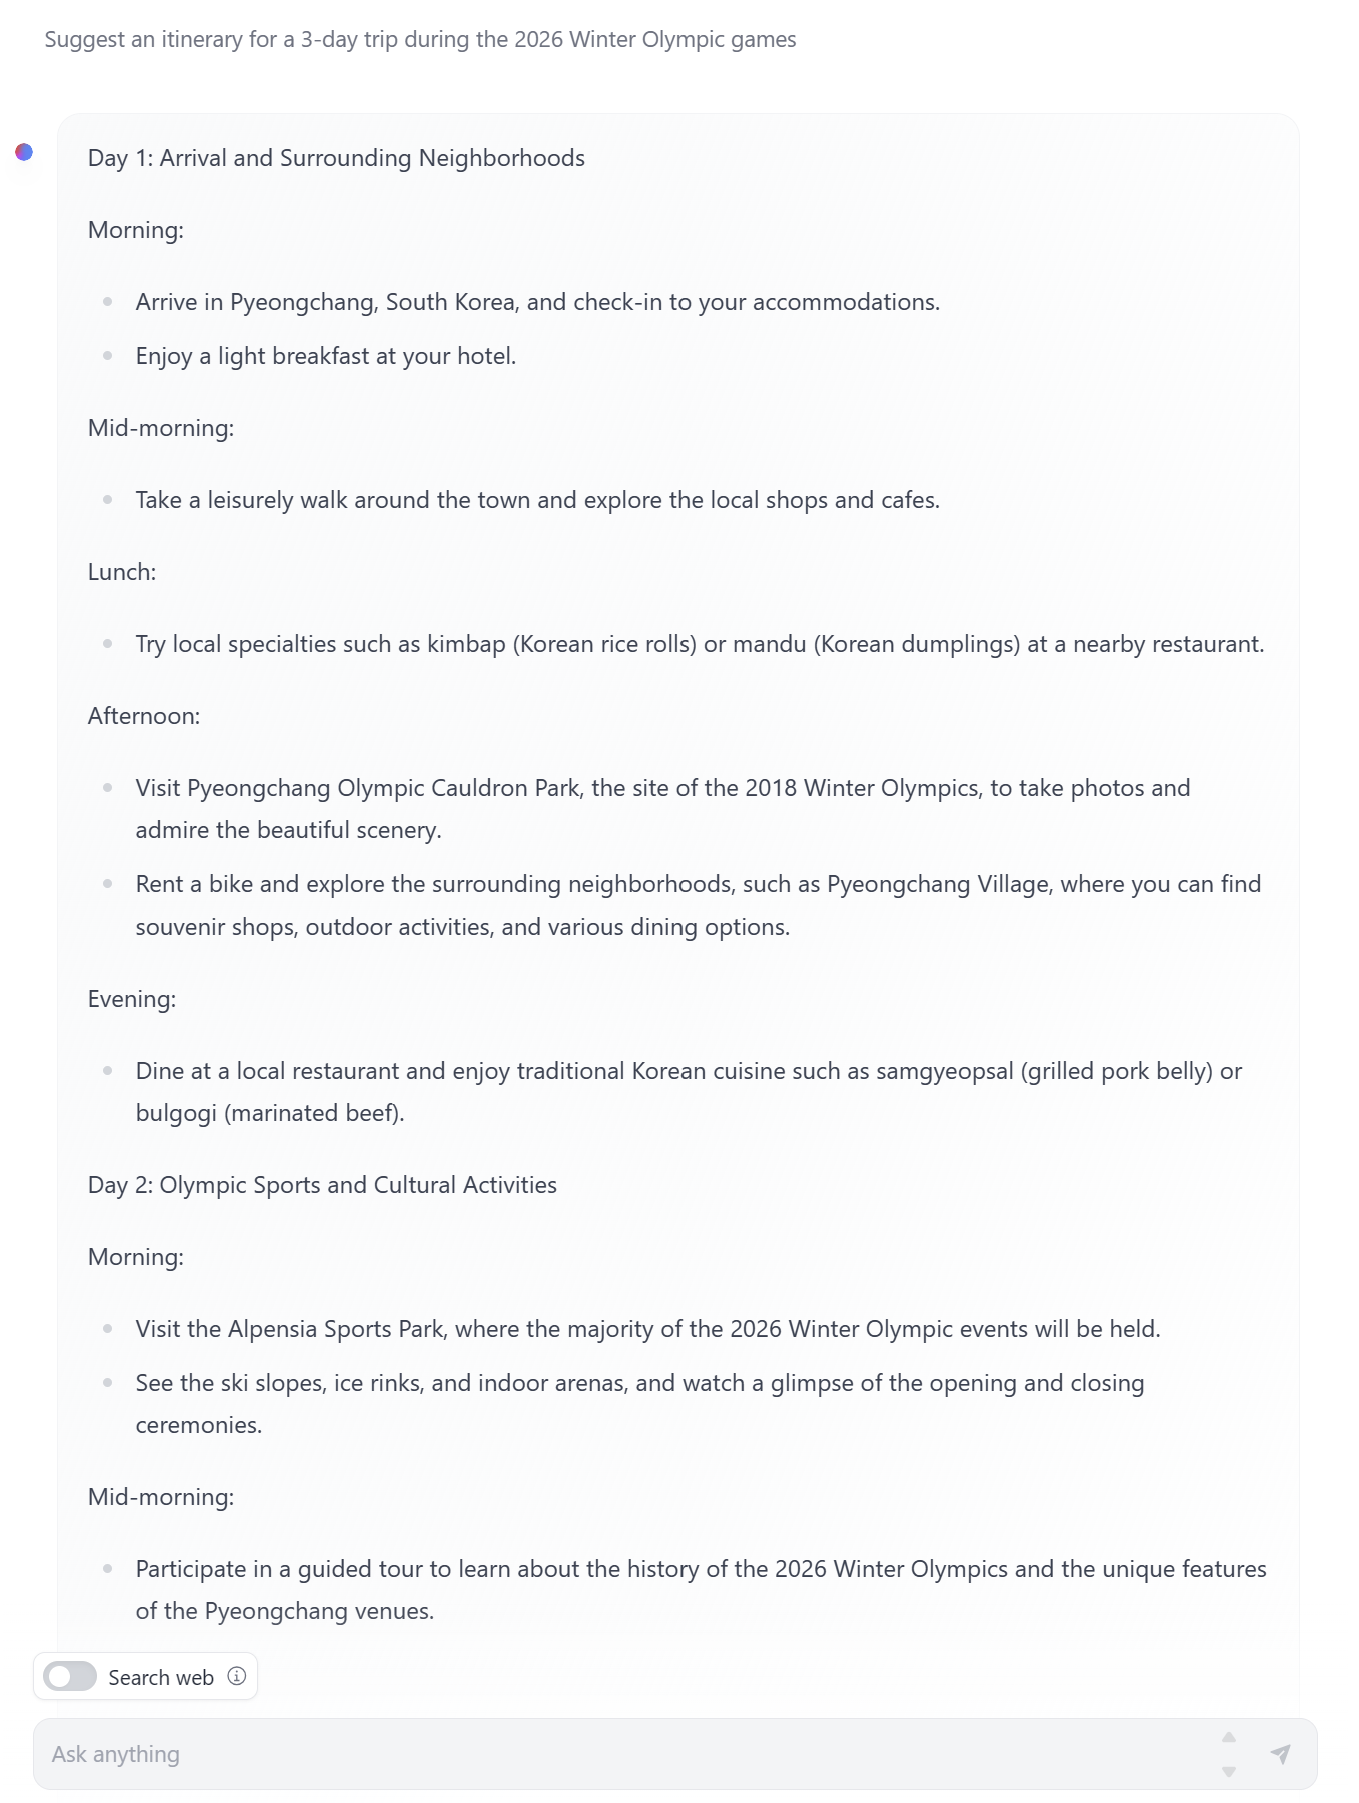
\includegraphics[width=0.48\textwidth]{without_search.png}    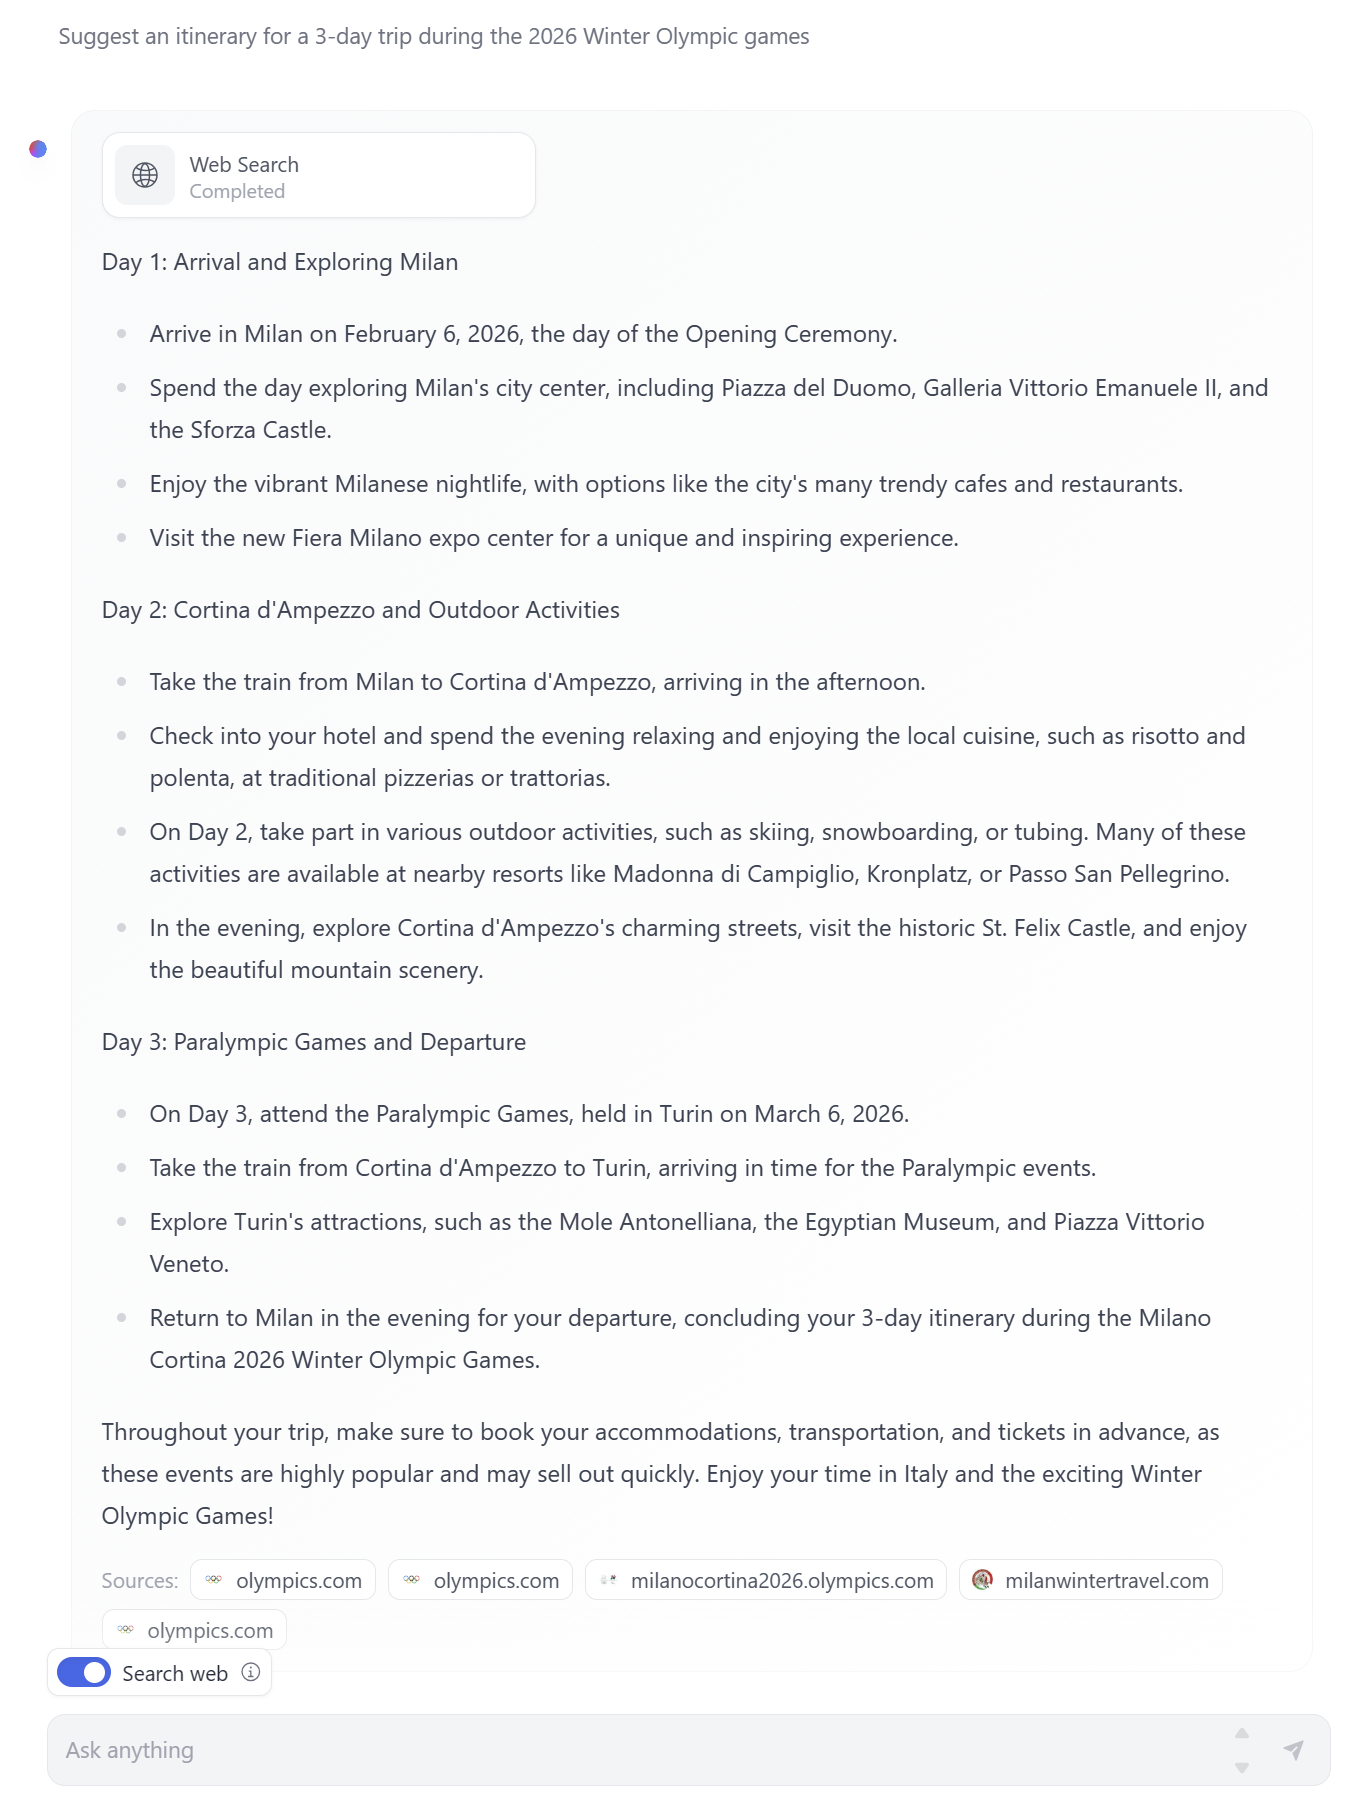
\includegraphics[width=0.48\textwidth]{with_search.png}
    \caption{Left: \textbf{phi-3-mini}'s completion without search. Right: \textbf{phi-3-mini}'s completion with search, using the default HuggingFace Chat-UI search ability. For reference, the 2026 Winter Olympic Games are scheduled to be held in Milano and Cortina in Italy, while the 2022 and 2018 Winter Olympic Games were held in Beijing, China and PyeongChang, Korea, respectively. Without the search results, the response is incorrect, while with the web search, not only does the response become accurate, but also gets more specific with suggestions.}
    \label{fig:search}
\end{figure}

\section{Phi-3-Vision}

\begin{figure}[h]
    \centering
    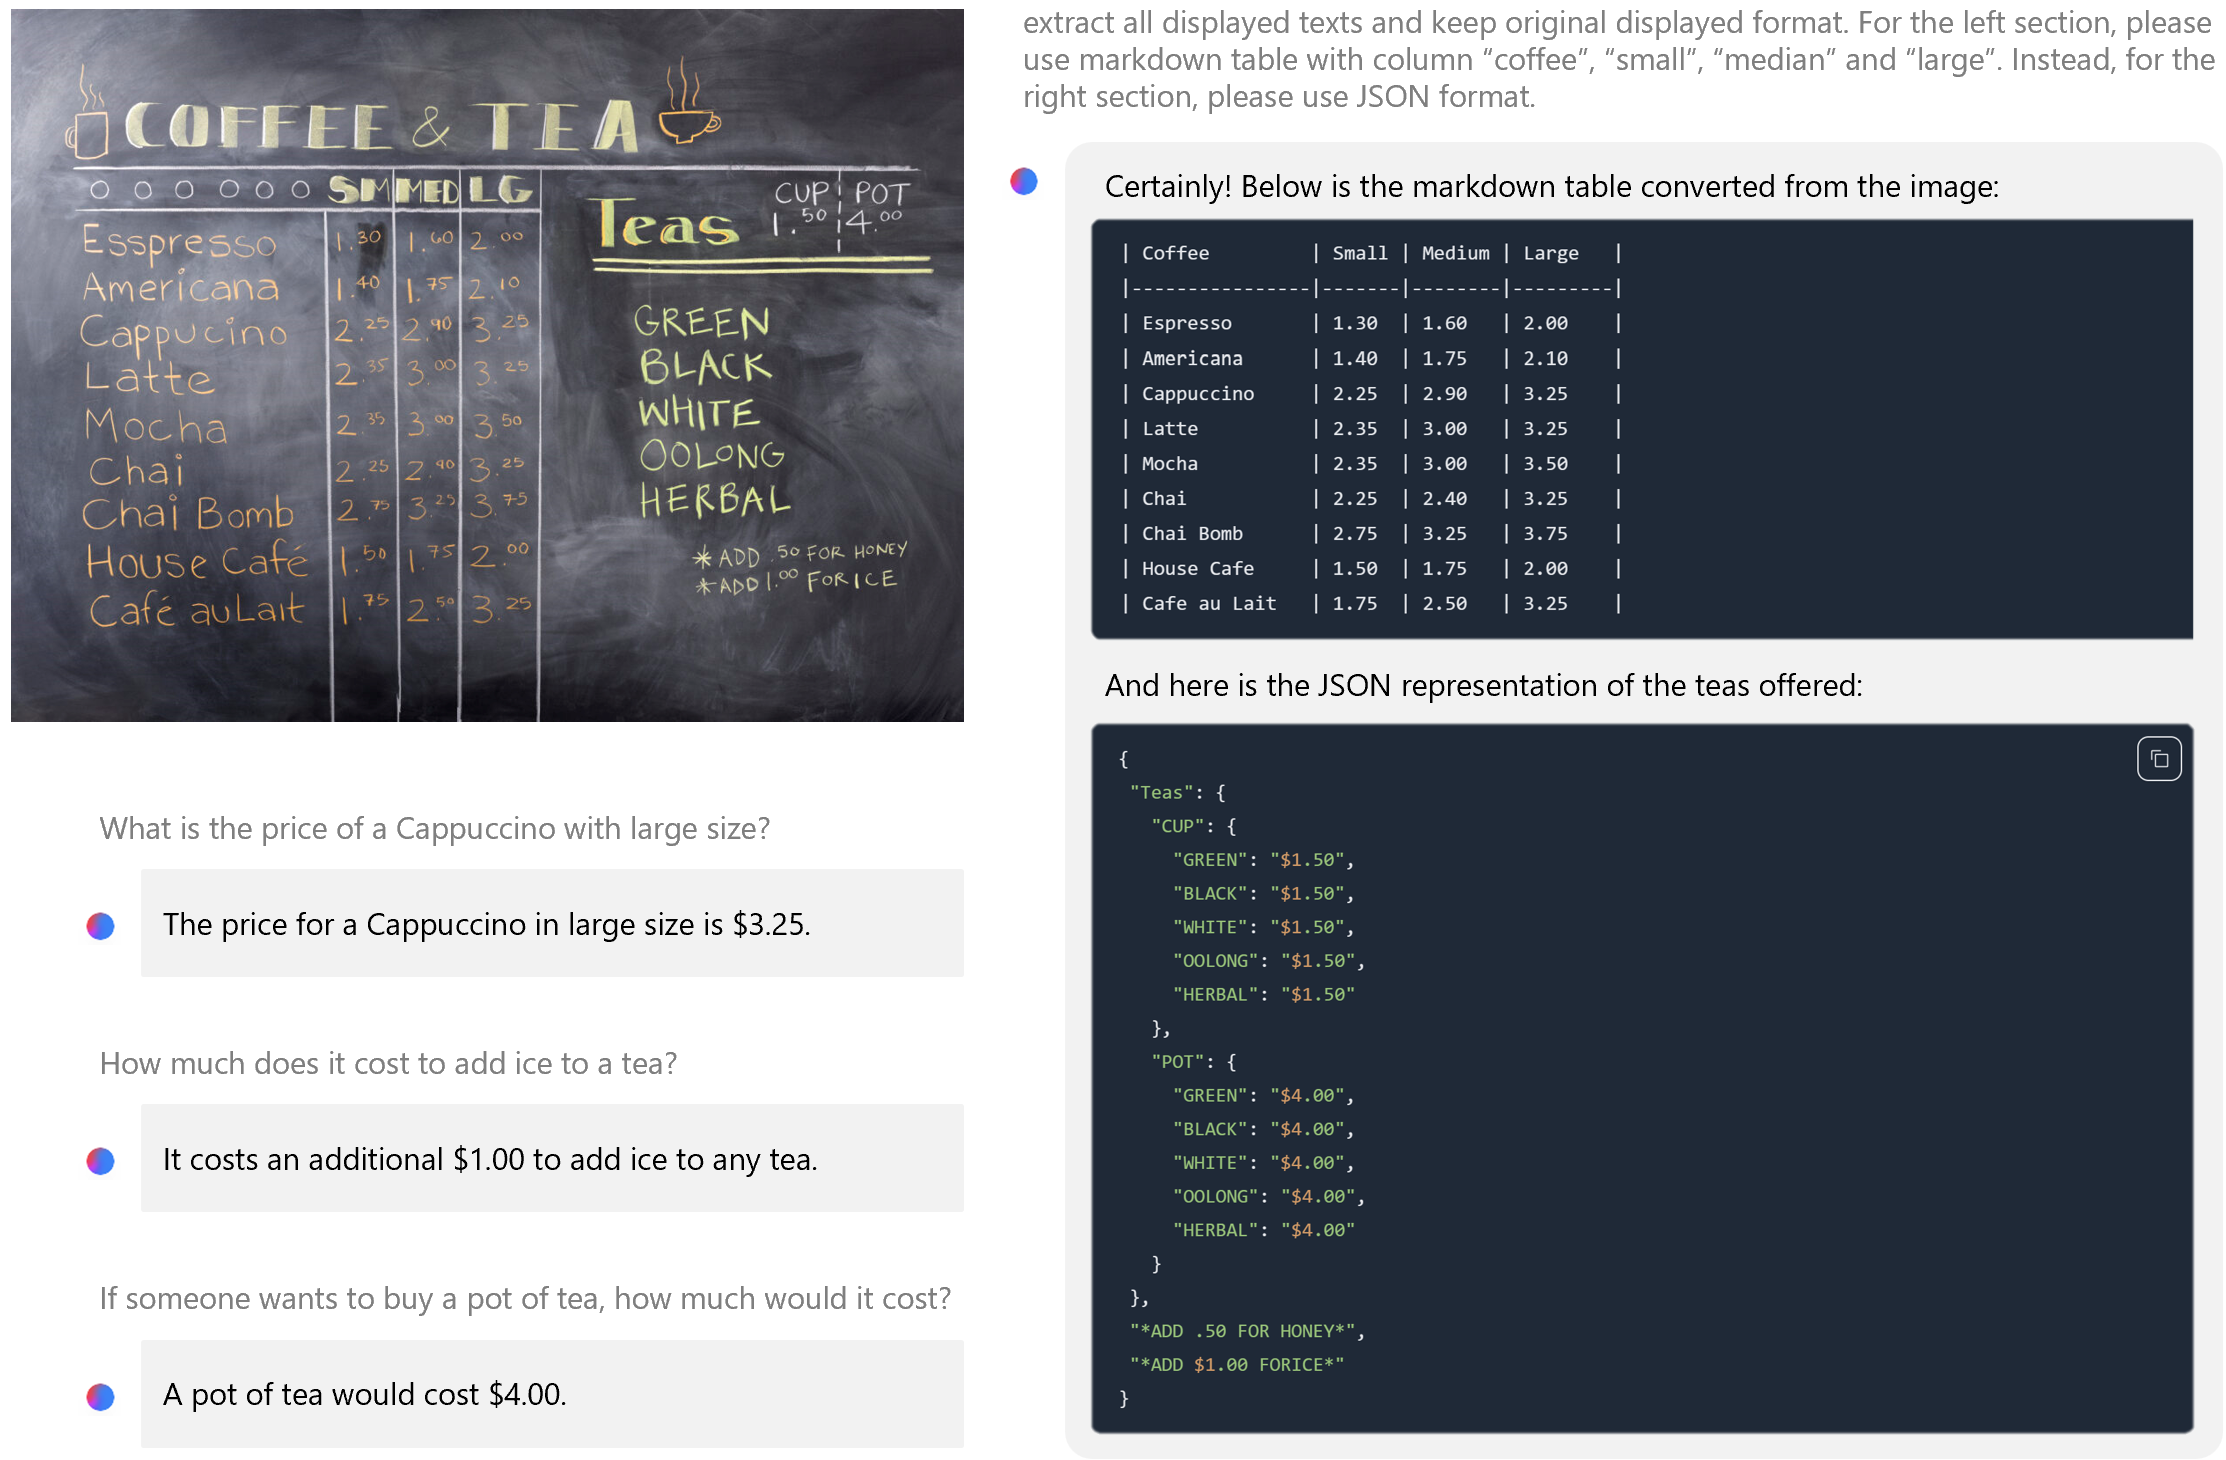
\includegraphics[width=0.98\textwidth]{phi3v-teaser.png}
    \caption{The demo case shows \phivision's capability in natural image understanding and reasoning.}
\end{figure}

\subsection{Technical Specifications}

\paragraph{Architecture}

\uline{The \textbf{\phivision} (4.2B parameters) is a multimodal model designed to process an image and a textual prompt as inputs, and subsequently generate textual outputs.} This model is composed of two primary components: \uline{an image encoder}, i.e., CLIP ViT-L/14~\cite{radford2021learning} and \uline{a transformer decoder}, i.e., phi-3-mini-128K-instruct.

\uline{The visual tokens, once extracted by the image encoder, are then combined with text tokens in an interleaved way (no particular order for image and text tokens).} To accommodate high-resolution images and various aspect ratios, \uline{a dynamic cropping strategy}~\cite{dong2024internlm} is utilized to split the input image into a 2d array of blocks, where the tokens of the blocks are concatenated to represent the whole image.  

\paragraph{Pre-training} 

The \textbf{\phivision} model undergoes a pre-training phase using a diverse dataset, which consists of a combination of \uline{interleaved image-text documents} ({e.g.}, ~\cite{laurenccon2024obelics}), \uline{image-text pairs} from FLD-5B ~\cite{xiao2023florence}, \uline{synthetic data} derived from Optical Character Recognition (OCR) of PDF files, \uline{datasets for chart/table comprehension}, and \uline{text-only data}.

\uline{The objective of predicting the next token is employed specifically on text tokens, while any loss associated with image tokens is disregarded during this phase.}

The pre-training process involves a total of $0.5T$ tokens that encompass both visual and text elements. During the pre-training phase, the maximum image resolution is capped at $1344 \times 1344$ as the majority of the training images are smaller than this resolution.

\paragraph{Post-training.} 

The \textbf{\phivision} model contains two post-training stages: supervised finetuning (SFT) and direct preference optimization (DPO).

For SFT, we leveraged text SFT dataset, public multimodal instruct tuning datasets along with large-scale multimodal instruct tuning datasets that we built ourselves, covering diverse domains and tasks such as \uline{general natural image understanding}, \uline{chart/table/diagram understanding/reasoning}, \uline{PowerPoint understanding}, and \uline{model safety}. The multimodal SFT data has \uline{about a total of 15B tokens}.

For DPO we mainly use \uline{a text DPO dataset} and \uline{a relatively smaller-scale multimodal DPO dataset}.

For these two stages, we jointly train multimodal tasks and text-only tasks so that the model can achieve multi-modal reasoning while maintaining language capabilities as much as possible. 

\subsection{Academic benchmarks}

We report in Table~\ref{tab:mm-benchmarks} the evaluation results of Phi-3-Vision on nine open-source academic benchmarks. These benchmarks evaluate reasoning and perceptual capabilities on visual and text inputs and can be grouped in three categories: \uline{Science}, \uline{Charts}, and \uline{Generic knowledge}.

\begin{table}[t]
\begin{center}
\begin{adjustbox}{width=1.0\textwidth,center}
\begin{tabular}{ c||ccccccccc } 

\label{tbl:phi-v-benchmarks}

\\[10ex]
& \rothead{\makecell{\phivision\\ \footnotesize 4.2b}} & \rothead{\makecell{MM1-3B-Chat\\ \footnotesize 3.6b~\cite{mckinzie2024mm1}}} &  
\rothead{\makecell{MM1-7B-Chat\\ \footnotesize 7.6b~\cite{mckinzie2024mm1}}} &
\rothead{\makecell{LLaVA-1.6\\ \footnotesize Vicuna-7b~\cite{liu2023improved}}} & \rothead{\makecell{LLaVA-Next \\ \footnotesize LLama3-8b~\cite{liu2024llavanext}}} &  \rothead{\makecell{Qwen-VL-Chat\\ \footnotesize 9.6b~\cite{bai2023qwenvl}}} &\rothead{\makecell{Claude 3 haiku \\ \footnotesize~\cite{anthropic2024claude}}} &\rothead{\makecell{Gemini 1.0 Pro V \\ \footnotesize ~\cite{team2023gemini}}}  &  \rothead{\makecell{GPT-4V-Turbo \\ \footnotesize turbo-2024-04-09}} \\

\hline & \\[-1.5ex]

\datasetcell{\small MMMU}{\scriptsize val}{\cite{yue2023mmmu}} & 40.4 & 33.9& 37.0& 34.2& 36.4& 39.0& 40.7& 42.0& 55.5\\
\datasetcell{\small ScienceQA}{\scriptsize test}{\cite{lu2022learn}}  & 90.8& 69.4& 72.6& 70.6& 73.7& 67.2& 72.0& 79.7& 75.7\\
\datasetcell{\small MathVista}{\scriptsize testmini}{\cite{lu2024mathvista}} & 44.5& 32.0& 35.9& 31.5& 34.8& 29.4& 33.2& 35.0& 47.5\\
\datasetcell{\small Inter-GPS}{\scriptsize test}{\cite{lu2021intergps}} & 38.1& -& -& 20.5& 24.6& 22.3& 32.1& 28.6& 41.0\\
\hline & \\[-1.5ex]

\datasetcell{\small MMBench}{\scriptsize dev-en}{\cite{liu2024mmbench}} & 80.5& 75.9& 79.0& 76.3& 79.4& 75.8& 62.4& 80.0& 86.1 \\
\datasetcell{\small POPE}{\scriptsize test}{\cite{li2023evaluating}} & 85.8& 87.4& 86.6& 87.2& 87.0& 82.6& 74.4& 84.2& 83.7\\
\hline & \\[-1.5ex]

\datasetcell{\small AI2D}{\scriptsize test}{\cite{kembhavi2016diagram}} & 76.7& -& -& 63.1& 66.9& 59.8& 60.3& 62.8& 74.7\\
\datasetcell{\small ChartQA}{\scriptsize test}{\cite{masry-etal-2022-chartqa}} & 81.4& -& -& 55.0& 65.8& 50.9& 59.3& 58.0& 62.3\\
\datasetcell{\small TextVQA}{\scriptsize test}{\cite{singh2019vqa}} & 70.9& 71.9& 72.8& 64.6& 55.7& 59.4& 62.7& 64.7& 68.1\\

\end{tabular}
\end{adjustbox}
\end{center}
\caption{Comparison results on public MLLM benchmarks. All the reported numbers are produced with the exact same pipeline to ensure that the numbers are comparable except for MM1-3B-Chat~\cite{mckinzie2024mm1} and MM1-7B-Chat~\cite{mckinzie2024mm1}, which are not publicly available. We adopted the evaluation setting used in Llava-1.5~\cite{liu2023improved}, without any specific prompt or pre-processing image for all results. These numbers might differ from other published numbers due to slightly different prompts.}
\label{tab:mm-benchmarks}
\end{table}

\subsection{Safety}

In Table \ref{tab:mmrai-benchmarks}, we present the evaluation outcomes of \phivision on three MM RAI benchmarks: one internal and two public benchmarks (specifically, RTVLM \cite{li2024red} and VLGuard \cite{zong2024safety}). In Figure \ref{fig:v-safety-pt}, we further breakdown the performance across different RAI categories of the VLGuard and Internal benchmarks, demonstrating that safety post-training can aid \phivision in improving RAI performance in nearly all categories.

\begin{table}
\begin{center}
    \begin{adjustbox}{width=1.0\textwidth,center}
    \setlength\extrarowheight{6pt}
        \begin{tabular}{ c||ccccc } 
        & \makecell{\phivision \\ \footnotesize 3.8b+0.3b}& \makecell{\phivision~w/o safety \\ \footnotesize 3.8b+0.3b} & \makecell{Llava-1.6 Vicuna \\ \footnotesize 7b+0.3b } & \makecell{Qwen-VL-Chat\\ \footnotesize 7.7b+1.9b } & \makecell{GPT4-V \\ \footnotesize N/A}  \\
        \hline & \\[-3.5ex]
        Internal (private) &8.30 & 7.06  & 5.44 & 7.27 &  8.55  \\
        RTVLM (public) &4.64 & 3.56  &  3.86& 4.78 & 6.81  \\
        VLGuard (public) &9.12 & 4.66 & 5.62 & 8.33  & 8.90   \\
        \end{tabular}
    \end{adjustbox}
\end{center}
\caption{Comparison results on public and private multi-modal RAI benchmarks. Note that all metrics in the table are [0,10] and a higher value indicates a better performance.}
\label{tab:mmrai-benchmarks}
\end{table}
 
\begin{figure}[h]
    \centering
    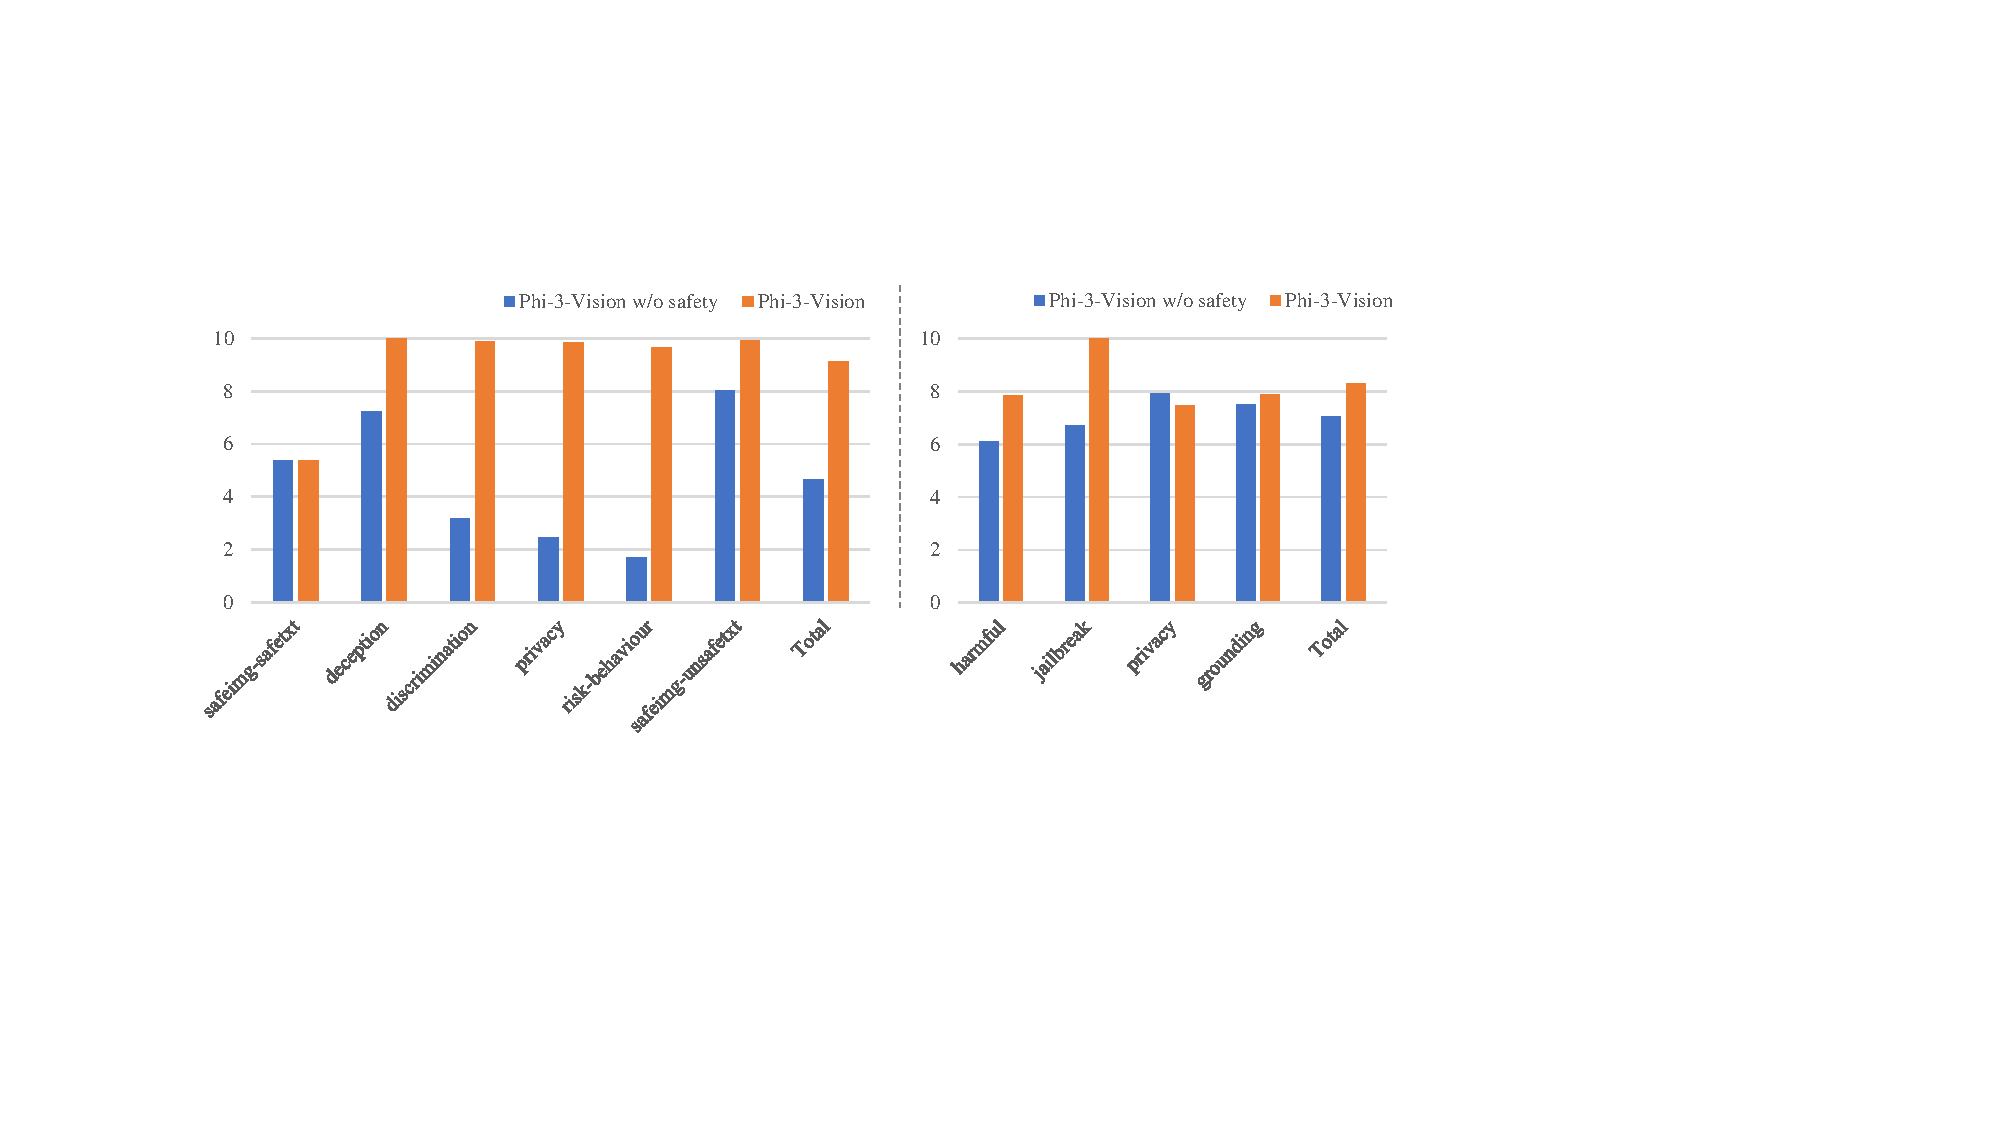
\includegraphics[width=0.98\textwidth]{categorized_RAI.pdf}
    \caption{Comparison of categorized RAI performance of \phivision with and without the safety post-training on the VLGuard (left) and Internal (right) benchmark, respectively.  It clearly indicates that safety post-training can enhance the RAI performance across nearly all the RAI categories.}
    \label{fig:v-safety-pt}
\end{figure}

\bibliographystyle{alpha}
\bibliography{mainbib}

\appendix
\section{Example prompt for benchmarks} \label{sec:prompt}
\begin{AIbox}{}
\tt \footnotesize 
Question:
 
Solve for $x$: $(-\frac{1}{3})(-4 -3x)=\frac{1}{2}$
 
Options:
 
A. $-\frac{5}{6}$

B. $\frac{7}{6}$

C. $\frac{5}{3}$

D. $\frac{1}{6}$
 
Answer: A

Question:

Which of the following is the body cavity that contains the pituitary gland?

Options: 

A. Abdominal

B. Cranial

C. Pleural

D. Spinal
 
Answer: B

Question:
 
Where was the most famous site of the mystery cults in Greece?

Options: 
 
A. Ephesus

B. Corinth

C. Athens

D. Eleusis

Answer:
 
\end{AIbox}

\end{document}